\documentclass{scrartcl}

\usepackage{amsmath}

\usepackage{tikz}
\usetikzlibrary{shapes, shapes.multipart, shapes.geometric}
\usetikzlibrary{positioning}

\newcommand*\circled[1]{\tikz[baseline=(char.base)]{
            \node[shape=circle,draw,inner sep=2pt] (char) {#1};}}

\begin{document}

\section{Method}

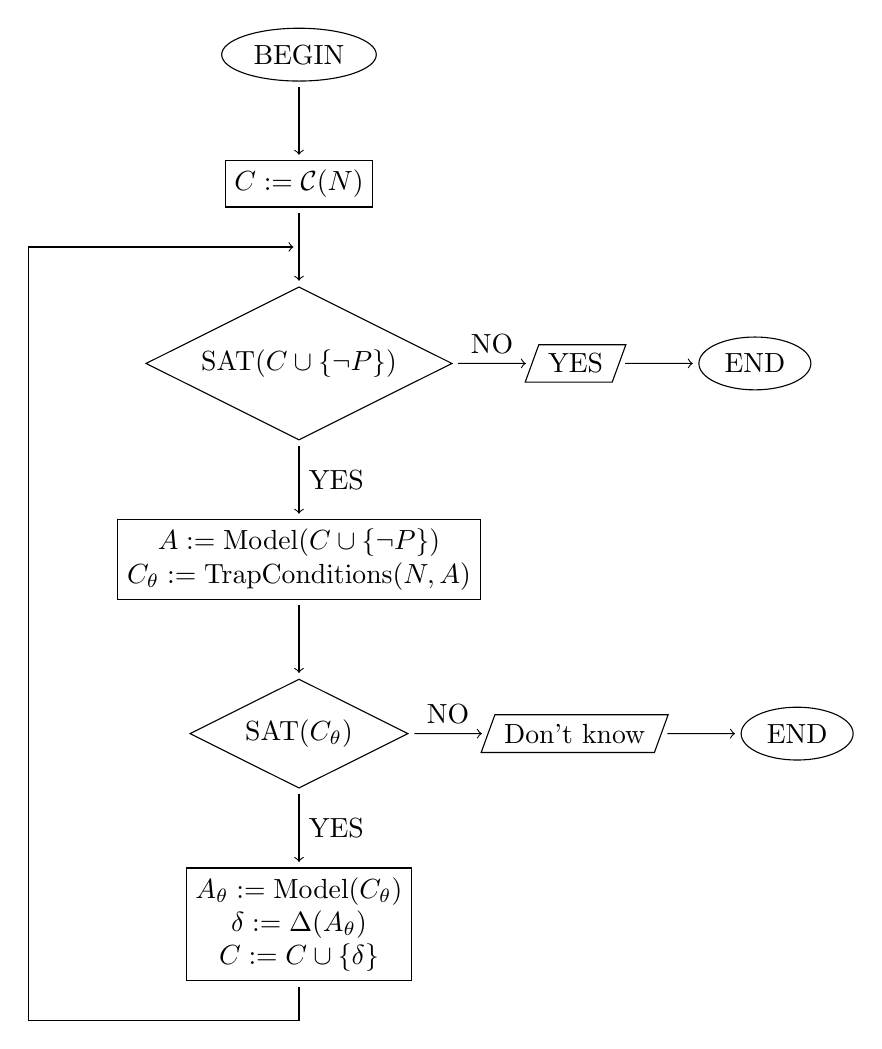
\begin{tikzpicture}[
    state/.style   = {draw, ellipse, aspect=2},
    action/.style  = {draw, rectangle, align=center},
    decision/.style= {draw, diamond, aspect=2, align=center},
    print/.style   = {draw, trapezium, trapezium left angle=70, trapezium right angle=-70},
    edge/.style    = {draw, ->, shorten >=2pt, shorten <=2pt},
  ]
  \node[state] (begin) {BEGIN};
  \node[action, below=of begin] (c) {$C:=\mathcal C(N)$};
  \node[decision, below=of c] (satc) {$\text{SAT}(C \cup \{\neg P\})$};
  \node[action, below=of satc] (modelc) {$A:=\text{Model}(C \cup \{\neg P\})$\\
                                   $C_{\theta}:=\text{TrapConditions}(N, A)$};
  \node[decision, below=of modelc] (satctheta) {$\text{SAT}(C_\theta)$};
  \node[action, below=of satctheta] (modelctheta) {$A_\theta:=\text{Model}(C_\theta)$\\
                                        $\delta:=\Delta(A_\theta)$\\
                                        $C:=C \cup \{\delta\}$};
  \node[print, right=of satc] (yes) {YES};
  \node[print, right=of satctheta] (dontknow) {Don't know};
  \node[state, right=of yes] (end1) {END};
  \node[state, right=of dontknow] (end2) {END};

  \draw (begin) edge[edge] (c);
  \draw (c) edge[edge] coordinate[pos=.5] (edgein) (satc);
  \draw (satc) edge[edge] node[above]{NO} (yes);
  \draw (yes) edge[edge] (end1);
  \draw (satc) edge[edge] node[right]{YES} (modelc);
  \draw (modelc) edge[edge] (satctheta);
  \draw (satctheta) edge[edge] node[above]{NO} (dontknow);
  \draw (dontknow) edge[edge] (end2);
  \draw (satctheta) edge[edge] node[right]{YES} (modelctheta);
  \draw[edge] (modelctheta.south) -- ([yshift=-0.5cm] modelctheta.south)
  -| ([xshift=-2cm] modelctheta.west) |- (edgein);
\end{tikzpicture}

\section{Constraints $C_0$}

%p_1 &=& 1 &{}-{}& u_1& u_2& u_3& u_4& u_5& &{}+{}& u_6&\\
%p_1 &=& 1 &{}-{}& u_1 &{}-{}& u_2 &{}-{}& u_3 &{}-{}& u_4 &{}-{}& u_5 &{}+{}& u_6 \\
%p_1 &=& 1 &     &     &     &     &     &     &     &     &     &     &     &     \\
\begin{alignat*}{15}
&& p_1 &{}={}& 1
  &{}-{}& u_1 &     &     &     &     &     &     &     &     &{}+{}& u_6 
  &     &     &     &     &     &     &     &     &     &     &     &     \\
&& p_2 &{}={}& 0
  &{}+{}& u_1 &{}-{}& u_2 &{}-{}& u_3 &     &     &     &     &     &     
  &     &     &     &     &     &     &     &     &     &     &     &     \\
&& p_3 &{}={}& 0
  &     &     &{}+{}& u_2 &{}+{}& u_3 &{}-{}& u_4 &{}-{}& u_5 &     &     
  &     &     &     &     &     &     &     &     &     &     &     &     \\
&& p_4 &{}={}& 0
  &     &     &     &     &     &     &{}+{}& u_4 &{}+{}& u_5 &{}-{}& u_6
  &     &     &     &     &     &     &     &     &     &     &     &     \\
&& q_1 &{}={}& 1
  &     &     &     &     &     &     &     &     &     &     &     &     
  &{}-{}& v_1 &     &     &     &     &     &     &     &     &{}+{}& v_6 \\
&& q_2 &{}={}& 0
  &     &     &     &     &     &     &     &     &     &     &     &    
  &{}+{}& v_1 &{}-{}& v_2 &{}-{}& v_3 &     &     &     &     &     &     \\
&& q_3 &{}={}& 0
  &     &     &     &     &     &     &     &     &     &     &     &     
  &     &     &{}+{}& v_2 &{}+{}& v_3 &{}-{}& v_4 &{}-{}& v_5 &     &     \\
&& q_4 &{}={}& 0
  &     &     &     &     &     &     &     &     &     &     &     &     
  &     &     &     &     &     &     &{}+{}& v_4 &{}+{}& v_5 &{}-{}& v_6 \\
&& (m_1=f) &{}={}& 1
  &{}-{}& u_1 &     &     &     &     &     &     &     &     &{}+{}& u_6     
  &     &     &     &     &     &     &     &     &     &     &     &     \\
&& (m_1=t) &{}={}& 0
  &{}+{}& u_1 &     &     &     &     &     &     &     &     &{}-{}& u_6     
  &     &     &     &     &     &     &     &     &     &     &     &     \\
&& (m_2=f) &{}={}& 1
  &     &     &     &     &     &     &     &     &     &     &     &     
  &{}-{}& v_1 &     &     &     &     &     &     &     &     &{}+{}& v_6 \\    
&& (m_2=t) &{}={}& 0
  &     &     &     &     &     &     &     &     &     &     &     &     
  &{}+{}& v_1 &     &     &     &     &     &     &     &     &{}-{}& v_6 \\    
&& (hold=1) &{}={}& 1
  &     &     &{}+{}& u_2 &     &     &     &     &     &     &     &     
  &     &     &     &     &{}-{}& v_3 &     &     &     &     &     &     \\
&& (hold=2) &{}={}& 0
  &     &     &{}-{}& u_2 &     &     &     &     &     &     &     &     
  &     &     &     &     &{}+{}& v_3 &     &     &     &     &     &     \\
&& p_4 &{}\ge{}& 1 \\
&& q_4 &{}\ge{}& 1 \\
&\forall p \in S \cup T:& p &{}\ge{}& 0
\end{alignat*}

\begin{align*}
  \delta_1 &= p_3 \lor q_2 \lor (m_2=f) \lor (hold=2) \\
  \delta_2 &= p_2 \lor q_3 \lor (m_1=f) \lor (hold=1)
\end{align*}

\section{$A_1$}

\begin{align*}
  p_1 &= 0 \\
  p_2 &= 0 \\
  p_3 &= 0 \\
  p_4 &= 1 \\
  q_1 &= 0 \\
  q_2 &= 0 \\
  q_3 &= 0 \\
  q_4 &= 1 \\
  (m_1=f) &= 0 \\
  (m_1=t) &= 1 \\
  (m_2=f) &= 0 \\
  (m_2=t) &= 1 \\
  (hold=1) &= 1 \\
  (hold=2) &= 0 \\
  u_1 &= 1 \\
  u_2 &= 0 \\
  u_3 &= 1 \\
  u_4 &= 0 \\
  u_5 &= 1 \\
  u_6 &= 0 \\
  v_1 &= 1 \\
  v_2 &= 1 \\
  v_3 &= 0 \\
  v_4 &= 1 \\
  v_5 &= 0 \\
  v_6 &= 0
\end{align*}

\section{$A_2$}

\begin{align*}
  p_1 &= 0 \\
  p_2 &= 0 \\
  p_3 &= 0 \\
  p_4 &= 1 \\
  q_1 &= 0 \\
  q_2 &= 0 \\
  q_3 &= 0 \\
  q_4 &= 1 \\
  (m_1=f) &= 0 \\
  (m_1=t) &= 1 \\
  (m_2=f) &= 0 \\
  (m_2=t) &= 1 \\
  (hold=1) &= 0 \\
  (hold=2) &= 1 \\
  u_1 &= 1 \\
  u_2 &= 0 \\
  u_3 &= 1 \\
  u_4 &= 1 \\
  u_5 &= 0 \\
  u_6 &= 0 \\
  v_1 &= 1 \\
  v_2 &= 0 \\
  v_3 &= 1 \\
  v_4 &= 1 \\
  v_5 &= 0 \\
  v_6 &= 0
\end{align*}

\section{$A_{\theta 1}$}
\begin{align*}
  bp_1 &= 0 \\
  bp_2 &= 0 \\
  bp_3 &= 1 \\
  bp_4 &= 0 \\
  bq_1 &= 0 \\
  bq_2 &= 1 \\
  bq_3 &= 0 \\
  bq_4 &= 0 \\
  b(m_1=f) &= 0 \\
  b(m_1=t) &= 0 \\
  b(m_2=f) &= 1 \\
  b(m_2=t) &= 0 \\
  b(hold=1) &= 0 \\
  b(hold=2) &= 1
\end{align*}

\section{$A_{\theta 2}$}
\begin{align*}
  bp_1 &= 0 \\
  bp_2 &= 1 \\
  bp_3 &= 0 \\
  bp_4 &= 0 \\
  bq_1 &= 0 \\
  bq_2 &= 0 \\
  bq_3 &= 1 \\
  bq_4 &= 0 \\
  b(m_1=f) &= 1 \\
  b(m_1=t) &= 0 \\
  b(m_2=f) &= 0 \\
  b(m_2=t) &= 0 \\
  b(hold=1) &= 1 \\
  b(hold=2) &= 0
\end{align*}

\section{$C_\theta$}

\circled{1}
\begin{align*}
  bp_1 &\implies (bp_2 \lor b(m_1=t)) \\
  bp_2 &\implies (bp_3 \lor b(hold=1)) \land (bp_3 \lor b(hold=1)) \\
  bp_3 &\implies (bp_4 \lor b(m_2=f)) \land (bp_4 \lor b(hold=2)) \\
  bp_4 &\implies (bp_1 \lor b(m_1=f)) \\
  bq_1 &\implies (bq_2 \lor b(m_2=t)) \\
  bq_2 &\implies (bq_3 \lor b(hold=2)) \land (bq_3 \lor b(hold=2)) \\
  bq_3 &\implies (bq_4 \lor b(m_1=f)) \land (bp_4 \lor b(hold=1)) \\
  bq_4 &\implies (bq_1 \lor b(m_2=f)) \\
  b(m_1=f) &\implies (bp_2 \lor b(m_1=t)) \land (bq_4 \lor b(m_1=f)) \\
  b(m_1=t) &\implies (bp_1 \lor b(m_1=f)) \\
  b(m_2=f) &\implies (bq_2 \lor b(m_2=t)) \land (bp_4 \lor b(m_2=f)) \\
  b(m_2=t) &\implies (bq_1 \lor b(m_2=f)) \\
  b(hold=1) &\implies (bq_3 \lor b(hold=2)) \land (bq_4 \lor b(hold=1)) \land (bp_3 \lor b(hold=1)) \\
  b(hold=2) &\implies (bp_3 \lor b(hold=1)) \land (bp_4 \lor b(hold=2)) \land (bq_3 \lor b(hold=2))
\end{align*}
\circled{2}
\begin{align*}
  bp_1 \lor bq_1 \lor b(m_1=f) \lor b(m_2=f) \lor b(hold=1)
\end{align*}
$\circled{3}_1$
\begin{align*}
  \neg bp_4 \land \neg bq_4 \land \neg b(m_1=t) \land
  \neg b(m_2=t) \land \neg b(hold=1)
\end{align*}
$\circled{3}_2$
\begin{align*}
  \neg bp_4 \land \neg bq_4 \land \neg b(m_1=t) \land
  \neg b(m_2=t) \land \neg b(hold=2)
\end{align*}

\end{document}
